\documentclass{article}
\usepackage[paperheight=11in,paperwidth=8.5in,margin=1in]{geometry}
\usepackage{fancyhdr}
\usepackage{mdwlist}
\usepackage{graphicx}
\setlength{\headheight}{15.2pt}
\pagestyle{fancy}

\begin{document}
\fancyhf{}
\lhead{Team Security Crawler}
\chead{Final Project Design}
\rhead{\today}

\begin{titlepage}
\begin{center}
{\huge Team Security Crawler}\\[2cm]
{\Large Final Project Design}\\[2cm]
{\large \today}\\[2cm]
\emph{Team Members:}\\
Alex \uppercase{Audretsch}\\
Michael \uppercase{Eaton}\\
Trevor \uppercase{Krenz}\\
Andrew \uppercase{Siegle}\\[1cm]
\emph{Client:}\\
Alan WLASUK\\
WDDinc.\\[1cm]
\emph{Advisor:}\\
Steve CHENOWETH

\end{center}
\end{titlepage}
\tableofcontents
\newpage
\section{Introduction}
403 Security is a web security firm based out of Indianapolis that is looking to increase its client base by way of a free, automated security scan that a potential client can request by way of a web service.  This service will save 403 employees valuable time and generate a sizeable number of clients for 403.
To this end, the Security Crawler system has been designed.  Because it is an automated service that anyone can access, it is restricted to analysis of page source, and cannot perform in-depth penetration scans.  However, a sizeable number of security vulnerabilites can be deduced from this data, such as out-of-date software and bad permissions in the html file tree.
This document contains updated designs and architectural models for the security crawler system, as well as discussions of sysetm design choices in light of GRASP and GoF patterns.  It includes the logical architecture of the system and finally an integration and acceptance testing plan for the system when it is deployed.

\newpage
\section{Analysis Models}
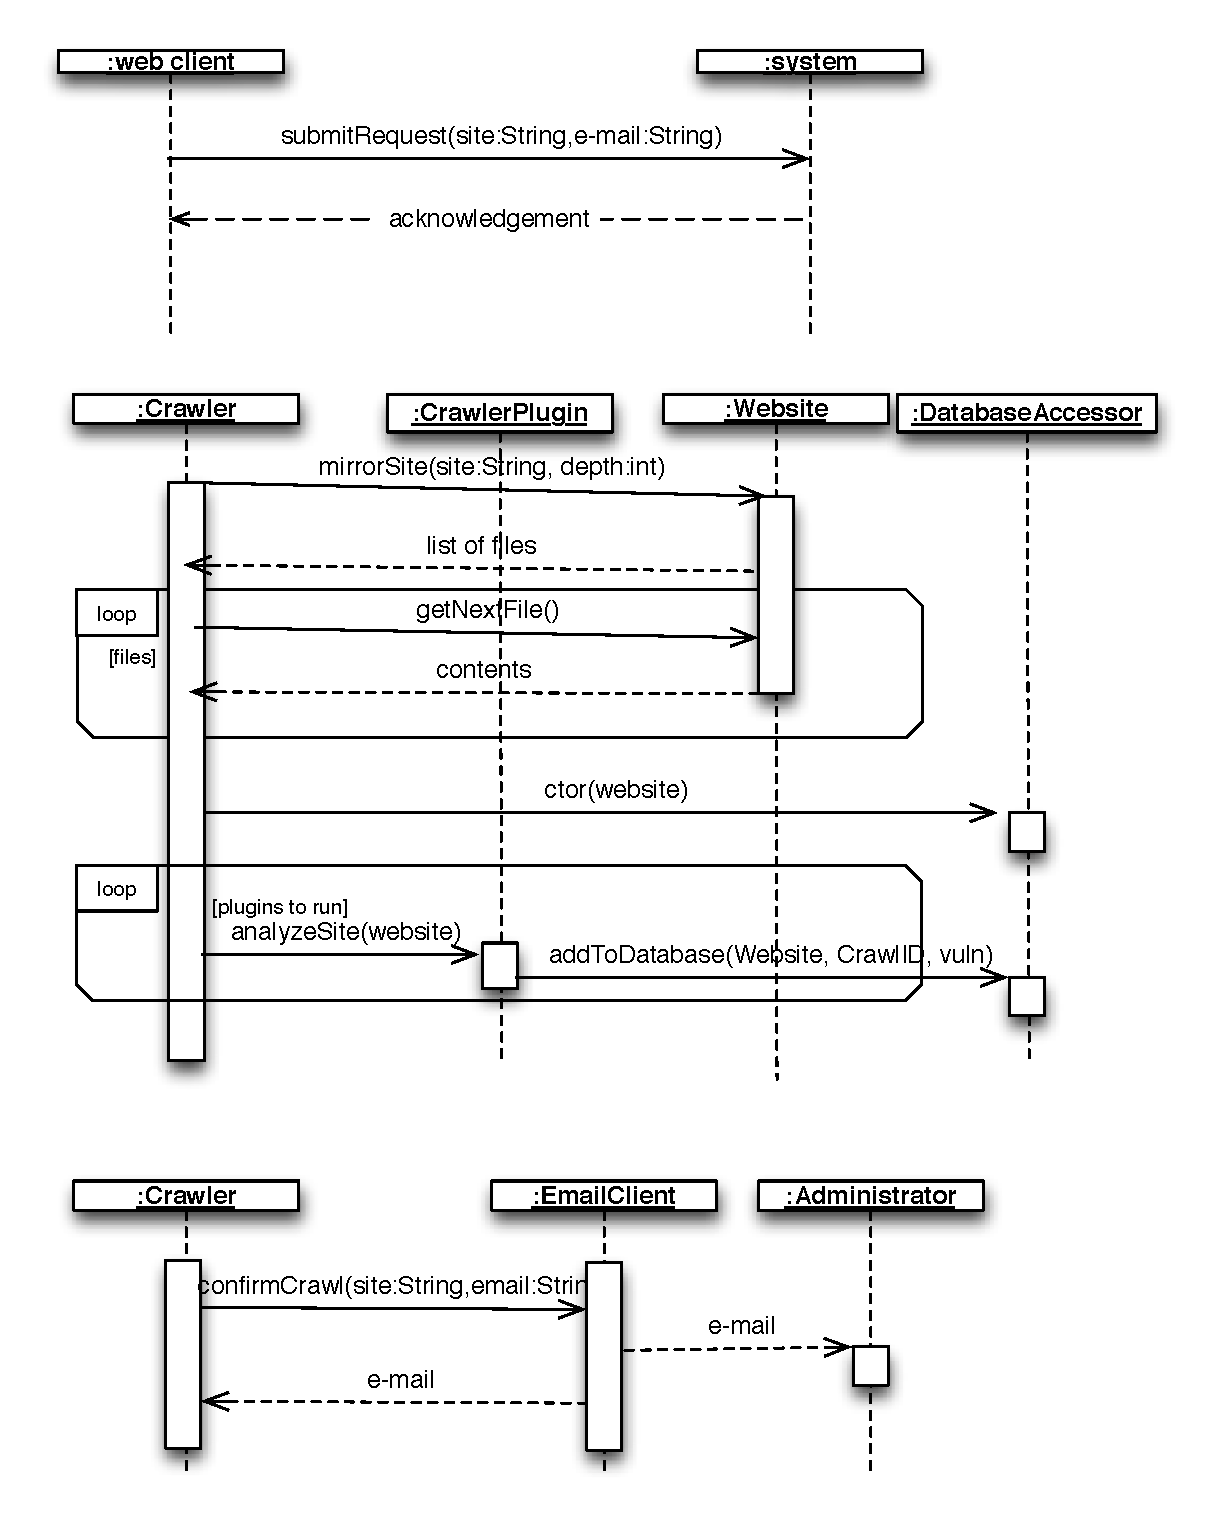
\includegraphics[width=\textwidth]{SeqDia}
\newpage
\section{Logical Architecture}
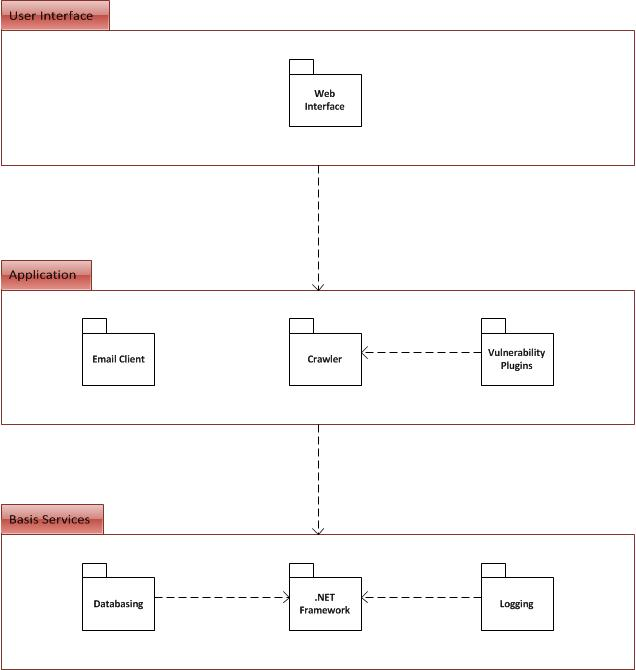
\includegraphics{LogArch}
\newpage
\section{Design with discussion}
\newpage
\section{Integration and Acceptance Test Plan}
\newpage
\section{Who Done What Table}
\begin{center}
\begin{tabular}{|l|c|}
\hline
Team member & Tasks \\ \hline
Alex Audretsch & 
\begin{minipage}{.4\textwidth}
\vspace{11pt}
\begin{itemize}
	\item Updated DCD
\end{itemize} 
\end{minipage} \\ \hline
Michael Eaton & 
\begin{minipage}{.4\textwidth}
\vspace{11pt}
\begin{itemize}
	\item Introduction
	\item Logical Architecture
\end{itemize} 
\end{minipage} \\ \hline
Trevor Krenz & 
\begin{minipage}{.4\textwidth}
\vspace{11pt}
\begin{itemize}
	\item Design with explanation (GRASP and GoF Principles)
\end{itemize} 
\end{minipage} \\ \hline
Andrew Siegle & 
\begin{minipage}{.4\textwidth}
\vspace{11pt}
\begin{itemize}
	\item Document Design
	\item Sequence Diagrams
\end{itemize} 
\end{minipage} \\ \hline
\end{tabular}
\end{center}


\end{document}